
了解代码有多少进行了测试有很大好处,这会对给定软件的测试情况有一个好的印象。还可以向开发人员提供关于测试未涉及的执行路径和边缘用例的提示。

有一些工具可以在C++中实现代码覆盖率,最流行的是GNU的Gcov。它已经存在多年了,可以很好地与GCC和Clang一起工作。它不能与微软的Visual Studio一起工作,但是使用Clang来构建和运行该软件为Windows提供了一个可行的替代方案。或者,可以使用工具OpenCppCoverage用MSVC构建,在Windows上获取覆盖数据。

Gcov生成的覆盖率信息可以通过Gcovr或LCOV工具在总结报告中收集。

\subsubsubsection{7.3.1\hspace{0.2cm}生成覆盖率报告}

本节中,将了解如何使用Gcovr创建这样的报告。生成代码覆盖率报告的大致方式如下:

\begin{enumerate}
\item 
要测试的程序和库用特殊的标志编译,因此需要公开覆盖率信息。

\item 
程序运行,覆盖率信息存储在一个文件中。

\item 
覆盖分析程序,如Gcovr或LCOV,分析覆盖文件并生成报告。

\item 
可以存储或进一步分析报告,以显示覆盖率的趋势。
\end{enumerate}

代码覆盖率的一个常见设置是,获得关于单元测试覆盖了多少项目代码的信息。为了做到这一点,必须使用必要的标志来编译代码,以便公开信息。

<LANG>\_COMPILER\_FLAGS缓存变量应该通过命令行传递给CMake。当使用GCC或Clang时,命令可能会是这样:

\begin{tcblisting}{commandshell={}}
cmake -S <sourceDir> -B <BuildDir> -DCMAKE_CXX_FLAGS=--coverage
\end{tcblisting}

另一种方法是定义各自的预设,详见第9章。构建覆盖测试时,在编译时启用调试信息并使用-Og标志禁用优化。此外,指定-fkeep-inline-functions和-fkeep-staticconsts编译器标志将阻止优化静态和内联函数(若从未使用过的话)。这将确保所有可能执行的分支都编译到代码中,否则,覆盖率报告可能会产生误导,特别是对于内联函数。

覆盖率报告不仅适用于单个可执行程序,还适用于库。然而,编译库时也必须打开覆盖率标志。

由于覆盖的编译器标志是全局的,选项会传递给使用\texttt{FetchContent}或\texttt{ExternalProject}添加的项目,这可能会增加编译时间。

启用覆盖标志的情况下,使用GCC或Clang编译源代码将为每个目标文件和可执行文件在构建目录中创建.gcno文件。这些文件包含Gcov的元信息,关于哪些调用和执行路径在各自的编译单元中可用。为了找出使用了哪些路径,必须运行程序。

对于想要找出测试的代码覆盖率的设置,运行ctest将生成覆盖率结果。或者,直接运行可执行程序也会产生相同的结果。运行启用覆盖的可执行程序将在构建目录中生成.gcda文件,其中包含有关各自目标文件中调用的信息。

生成这些文件后,运行Gcovr将创建关于覆盖率的信息。默认情况下,Gcovr将信息输出到标准输出,也可以生成HTML页面、JSON文件或SonarQube报告。

\begin{tcblisting}{commandshell={}}
gcovr -r <SOURCE_DIR> <BINARY_DIR> -html
\end{tcblisting}

这样会产生一个HTML文件:

\begin{center}
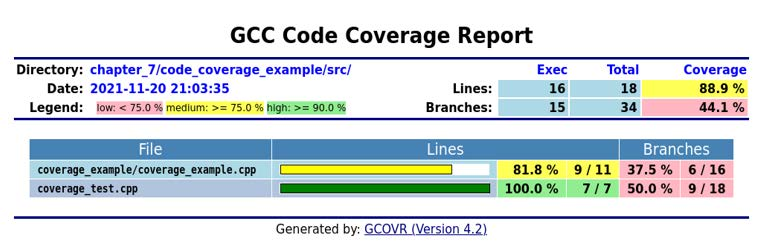
\includegraphics[width=0.6\textwidth]{content/2/chapter7/images/1.jpg}\\
图7.1 覆盖测试运行的示例输出
\end{center}

Gcovr的另一个替代方案是LCOV,其工作原理与Gcovr非常相似。与Gcovr相比,LCOV不能直接产生HTML或XML输出,而是将覆盖率信息以中间格式组合,然后可由各种转换器使用。为了生成HTML输出,经常使用genhtml。要使用LCOV生成报告,命令如下所示:

\begin{tcblisting}{commandshell={}}
lcov -c -d <BINARY_DIR> -o <OUTPUT_FILE>
genhtml -o <HTML_OUTPUT_PATH> <LCOV_OUTPUT>
\end{tcblisting}

使用LCOV生成的覆盖率报告可能如下所示:

\begin{center}
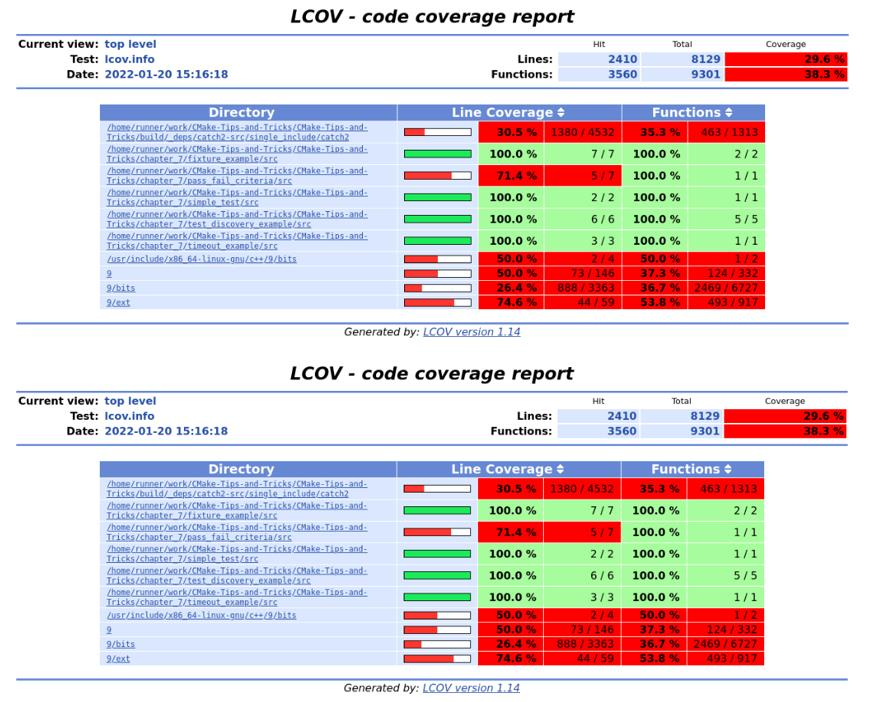
\includegraphics[width=0.7\textwidth]{content/2/chapter7/images/2.jpg}\\
图7.2 使用LCOV生成的覆盖率报告示例
\end{center}

这只会为最后一次运行创建覆盖率报告。若想将它们组合成一个时间序列,以查看代码覆盖率是上升还是下降,可以使用各种CI工具,如Codecov和Cobertura来完成此工作。这些工具通常可以解析来自Gcovr或LCOV的输出,并将其组装成显示覆盖率趋势。Gcovr的详细文档可参见\url{https://gcovr.com/en/stable/}。

\subsubsubsection{7.3.2\hspace{0.2cm}为MSVC创建覆盖率报告}

当使用Microsoft Visual Studio构建软件时,OpenCppCoverage工具是Gcov的替代方案,其工作原理是分析MSVC编译器生成的程序数据库(.pdb),而不是用标志编译源代码。为单个可执行文件生成HTML覆盖率报告的命令可能如下所示:

\begin{tcblisting}{commandshell={}}
OpenCppCoverage.exe --export_type html:coverage.html --
  MyProgram.exe arg1 arg2
\end{tcblisting}

由于这只会为单个可执行文件生成覆盖率报告,OpenCppCoverage可以读取前几轮的输入,并将它们组合成如下报告:

\begin{tcblisting}{commandshell={}}
OpenCppCoverage.exe --export_type binary:program1.cov --
  program1.exe
OpenCppCoverage.exe --export_type binary:program2.cov --
  program2.exe
OpenCppCoverage.exe --input_coverage=program1.cov --input_
coverage= program2.cov --export_type html:coverage.html
\end{tcblisting}

这将把前两次运行的输出合并到一个公共报告中。要使用覆盖率信息,export\_type选项必须是binary。

覆盖率报告的常见用途是找出项目中定义的测试覆盖了多少代码,由于CTest将运行测试作为子进程,-{}-cover\_children选项必须传递给OpenCppCoverage。为了避免为系统库生成覆盖率报告,可能需要添加一个模块和一个源过滤器。命令看起来像这样:

\begin{tcblisting}{commandshell={}}
OpenCppCoverage.exe --cover_children --modules <build_dir> --
  sources <source_dir> -- ctest.exe --build-config Debug
\end{tcblisting}

这种方法的小缺点是覆盖报告将包括CTest本身的覆盖报告。生成的HTML报告可能像这样:

\begin{center}
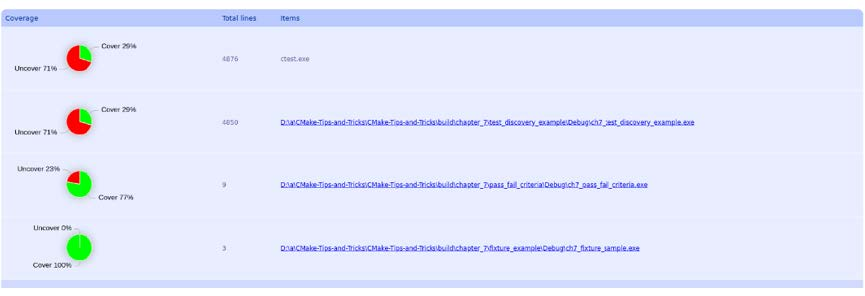
\includegraphics[width=0.8\textwidth]{content/2/chapter7/images/3.jpg}\\
图7.3 使用OpenCppCoverage生成的覆盖率报告
\end{center}

命令行之外的另一种选择是使用Visual Studio的插件,插件可以在Visual Studio市场上找到:\url{https://marketplace.visualstudio.com/items?itemName=OpenCppCoverage.OpenCppCoveragePlugin}。

完整的文档,请参考OpenCppCoverage的GitHub页面:
\url{https://github.com/OpenCppCoverage/OpenCppCoverage}

了解所提供的测试覆盖了多少代码,是代码质量非常重要的信息。在许多受监管的行业(如医疗技术、航空或汽车行业)中,监管机构可能会要求提供代码覆盖率报告。然而,仅仅知道执行了多少代码显然是不够的,底层代码的质量更加重要。一些编译器在消毒器的帮助下,提供有用的工具来检测代码中的常见错误。下一节中,将学习如何使用CMake使用和应用消毒器。

























